% !TEX root = ../thesis-example.tex
%
\chapter{Latex Sandbox}
\label{ch:latex_sandbox}

First use \gls{NIME}\\
subsequent \gls{NIME}

\gls{IRCAM} puis \gls{IRCAM}\\
\gls{OSC} puis \gls{OSC}\\
\gls{MIDI} puis \gls{MIDI}\\
\gls{MPE} puis \gls{MPE}\\
\gls{GRM} puis \gls{GRM}\\
\gls{DMI} puis \gls{DMI}\\


Exemple de \hl{texte surligné}. Et voilà


\begin{titlebox}{A physical explanation of the \emph{dynamic matrix}}
A physical explanation the \emph{dynamic matrix}\\
lots of text\\
a new line\\
equation
where  is a unitary matrix (each column is one of the eigenvectors of the dynamic matrix is the product of the number of particlces, and the number of dimensions,
\end{titlebox}

\begin{notebox}{This is just a test}
A physical explanation the \emph{dynamic matrix}\\
lots of text\\
a new line\\
equation
where  is a unitary matrix (each column is one of the eigenvectors of the dynamic matrix is the product of the number of particlces, and the number of dimensions,
\end{notebox}

\begin{notebox}
A physical explanation the \emph{dynamic matrix}\\
lots of text\\
a new line\\
equation
where  is a unitary matrix (each column is one of the eigenvectors of the dynamic matrix is the product of the number of particlces, and the number of dimensions,
\end{notebox}

\blindtext

\section*{figures}

\subsection*{figure simple dépassant sur les marges}

\begin{figure}[htb]
	\centerline{
		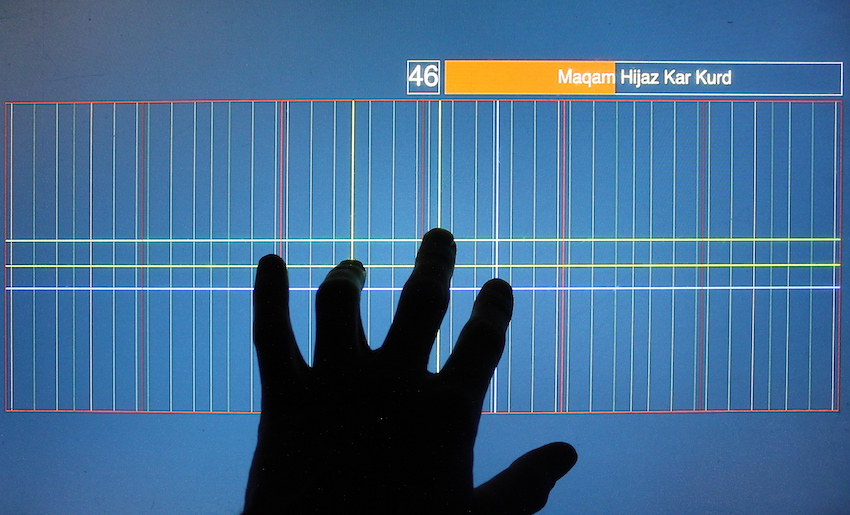
\includegraphics[width=1.2\textwidth]{gfx/06_visual_representation/mpTUI_pitchgrid_72dpi.png}
	}
	\caption{à gauche : évolution de la forme des ouïes du violon d'après \cite{nia_evolution_2015}. à droite : Extrait du brevet de J. Djalma sur \iquote{l'amélioration du clétage des flûtes de Boehm}, 1908.}
	\label{fig:sandbox:single}
\end{figure}

ou bien

\begin{center}
  \makebox[\textwidth]{
  	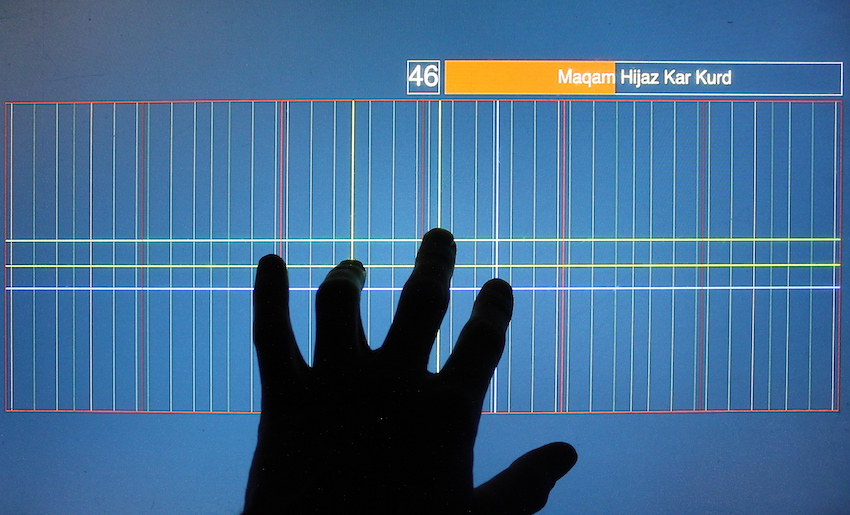
\includegraphics[width=\paperwidth]{gfx/06_visual_representation/mpTUI_pitchgrid_72dpi.png}
  	}
\end{center}

\subsection*{figures multiples, dépassant sur les marges}

\begin{figure}
	\makebox[\linewidth][c]{%
		\begin{subfigure}[b]{.6\textwidth}
			\centering
			
\includegraphics[width=.95\textwidth]{gfx/06_visual_representation/f-hole.png}
			\caption{a test subfigure}
		\end{subfigure}%
		\begin{subfigure}[b]{.6\textwidth}
			\centering
			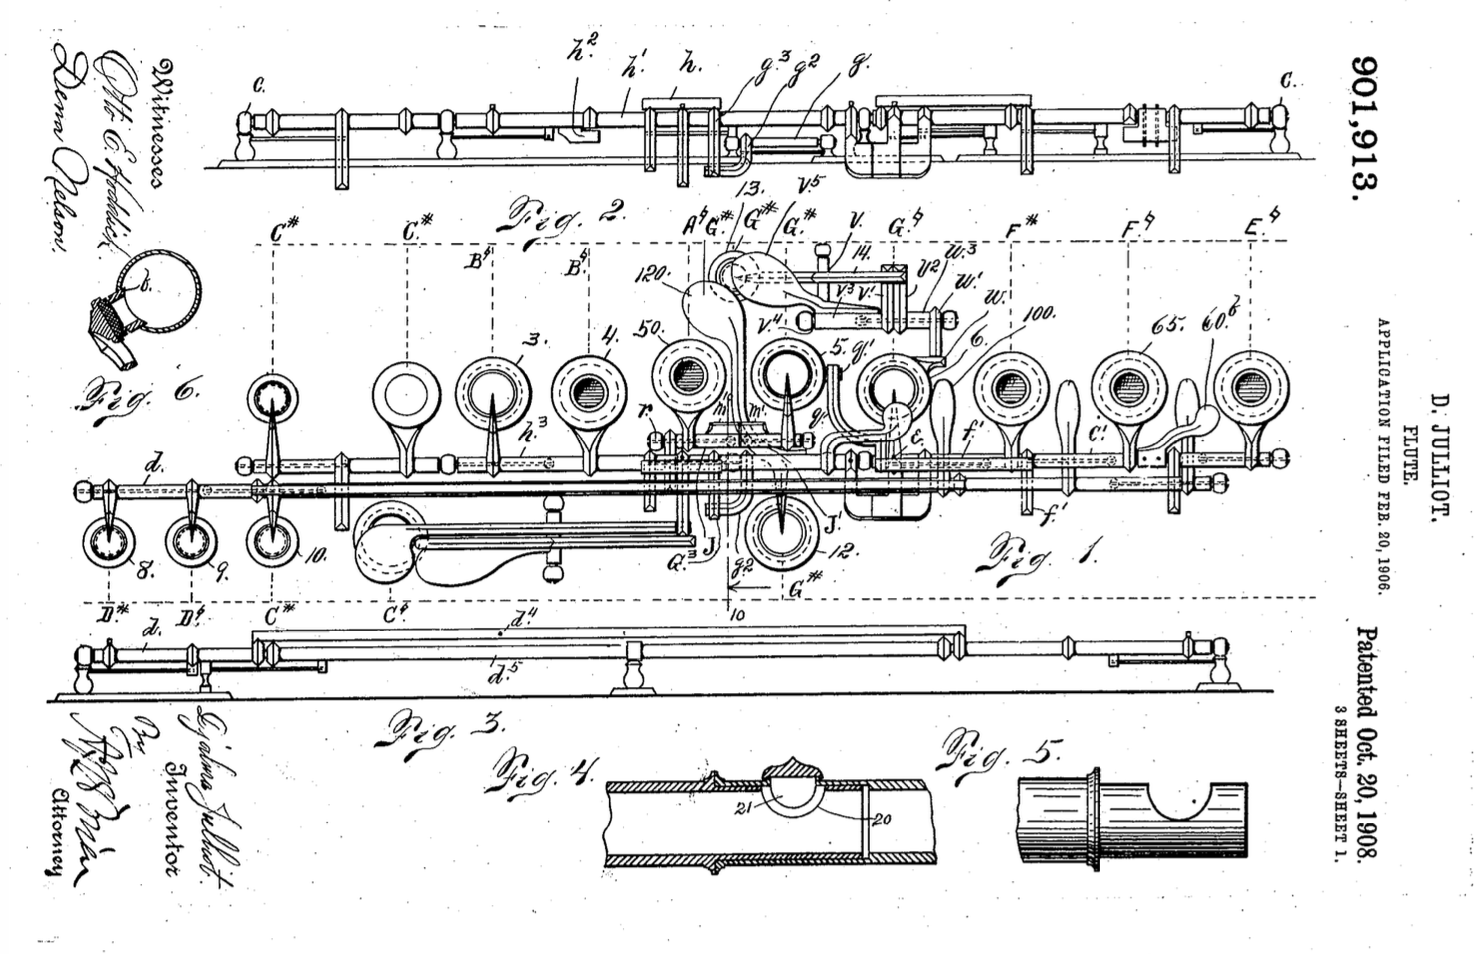
\includegraphics[width=.95\textwidth]{gfx/06_visual_representation/Julliot_patent.png}
			\caption{a test subfigure}
		\end{subfigure}%
	}\\
	\makebox[\linewidth][c]{%
		\begin{subfigure}[b]{.6\textwidth}
			\centering
			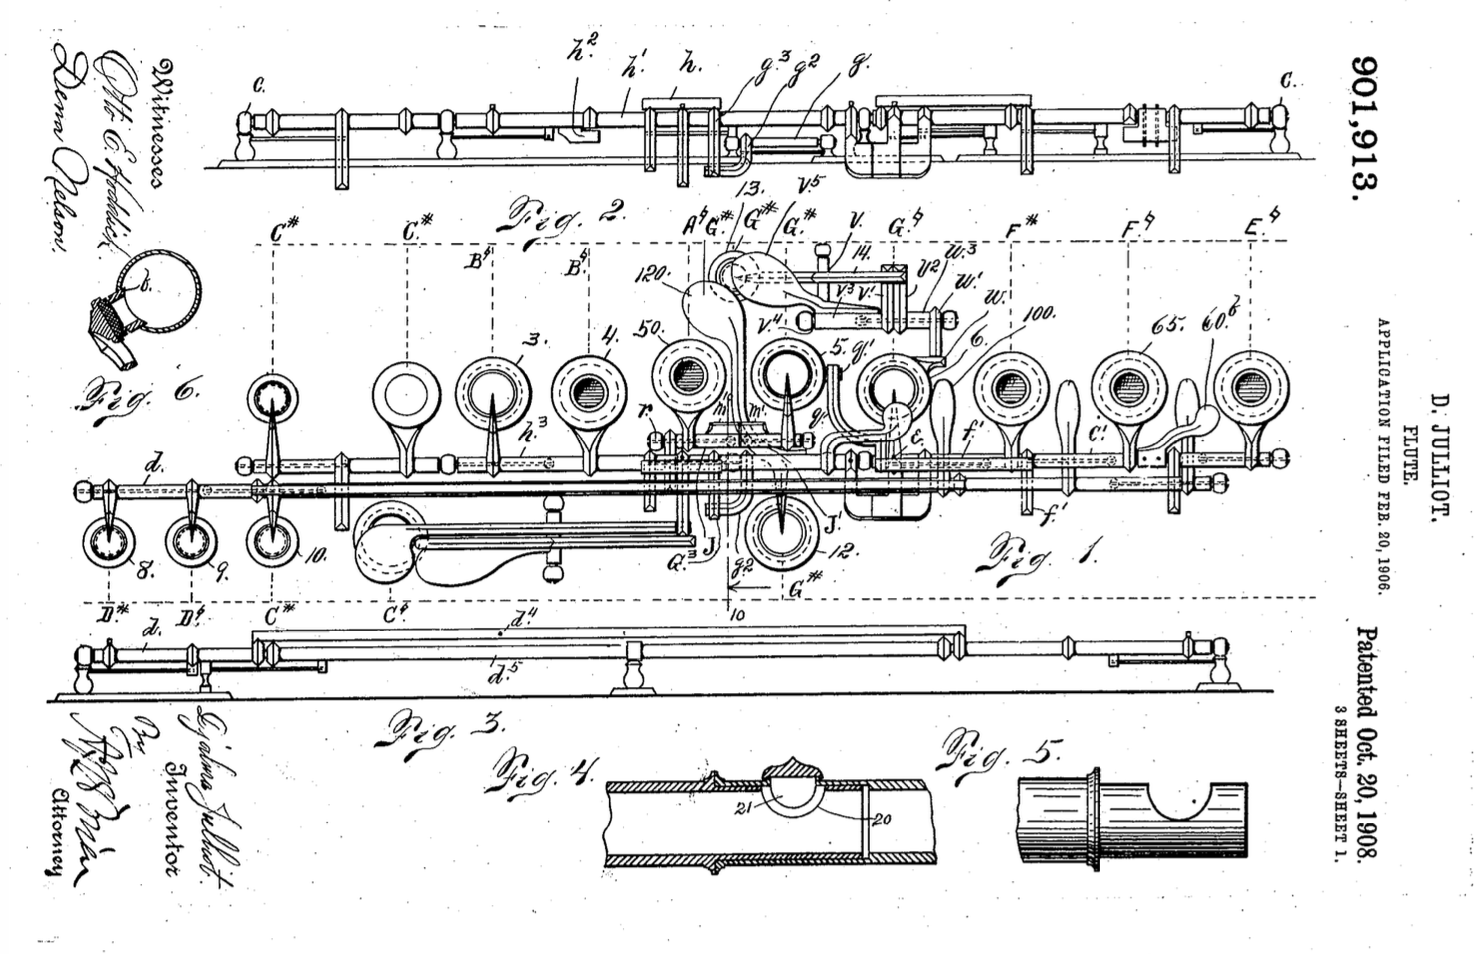
\includegraphics[width=.95\textwidth]{gfx/06_visual_representation/Julliot_patent.png}
			\caption{a test subfigure}
		\end{subfigure}%
		\begin{subfigure}[b]{.6\textwidth}
			\centering
			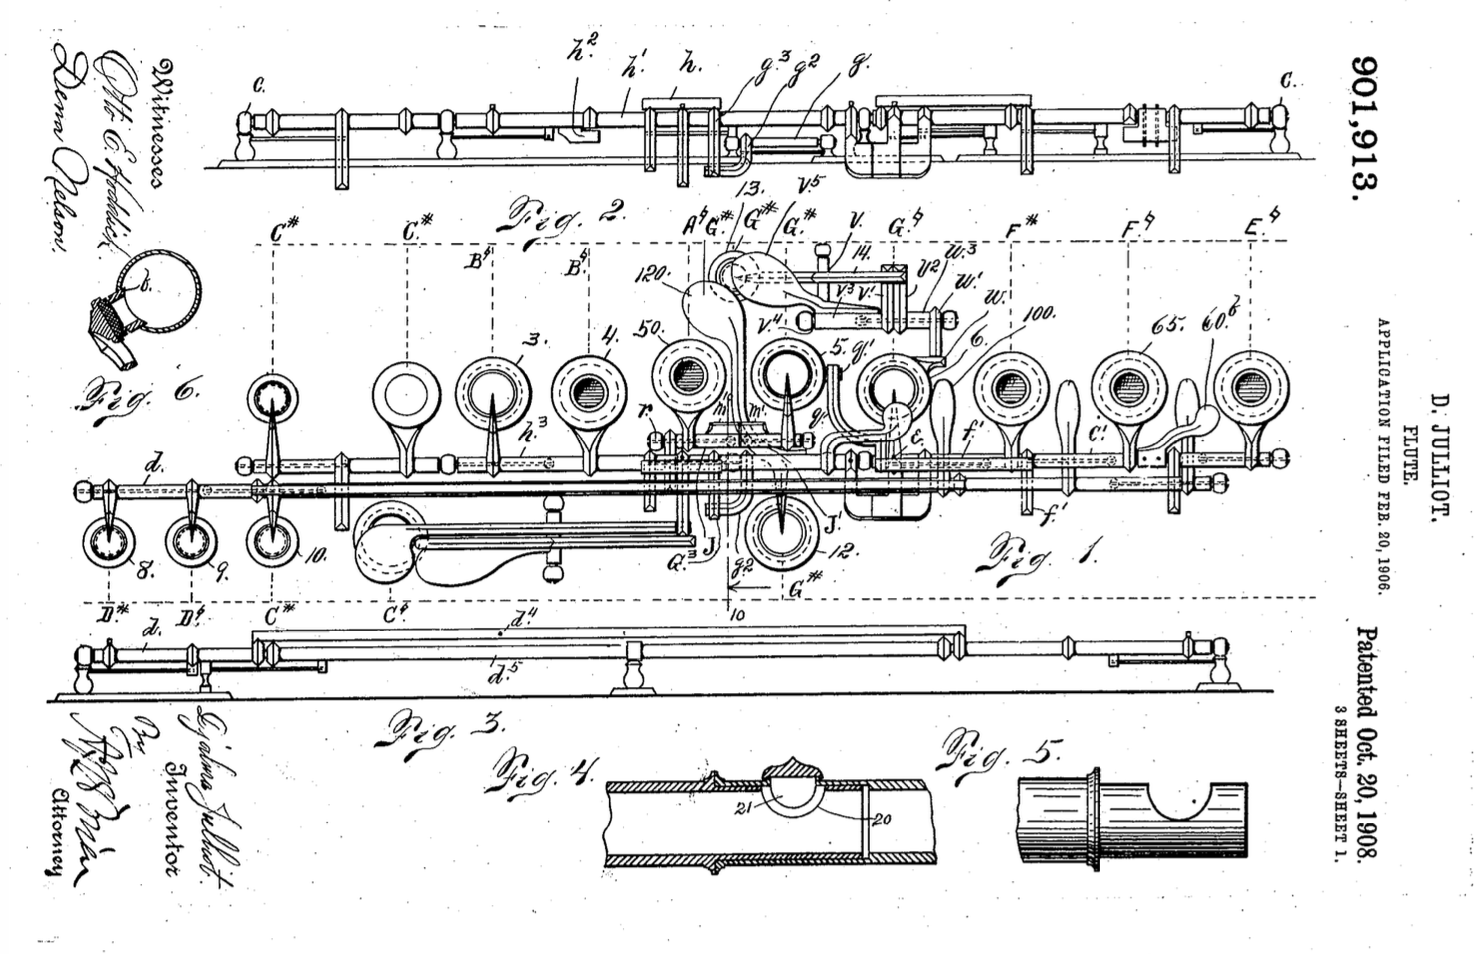
\includegraphics[width=.95\textwidth]{gfx/06_visual_representation/Julliot_patent.png}
			\caption{a test subfigure}
		\end{subfigure}%
	}
	\caption{A figure with four subfigures}
\end{figure}

/blindtext

\begin{figure}[h]
	\centering
	\begin{minipage}{.45\linewidth}
	    
\includegraphics[width=\linewidth]{gfx/06_visual_representation/f-hole.png}
	    \caption{First caption}
	    \label{img1}
	\end{minipage}
	\hspace{.05\linewidth}
	\begin{minipage}{.45\linewidth}
	    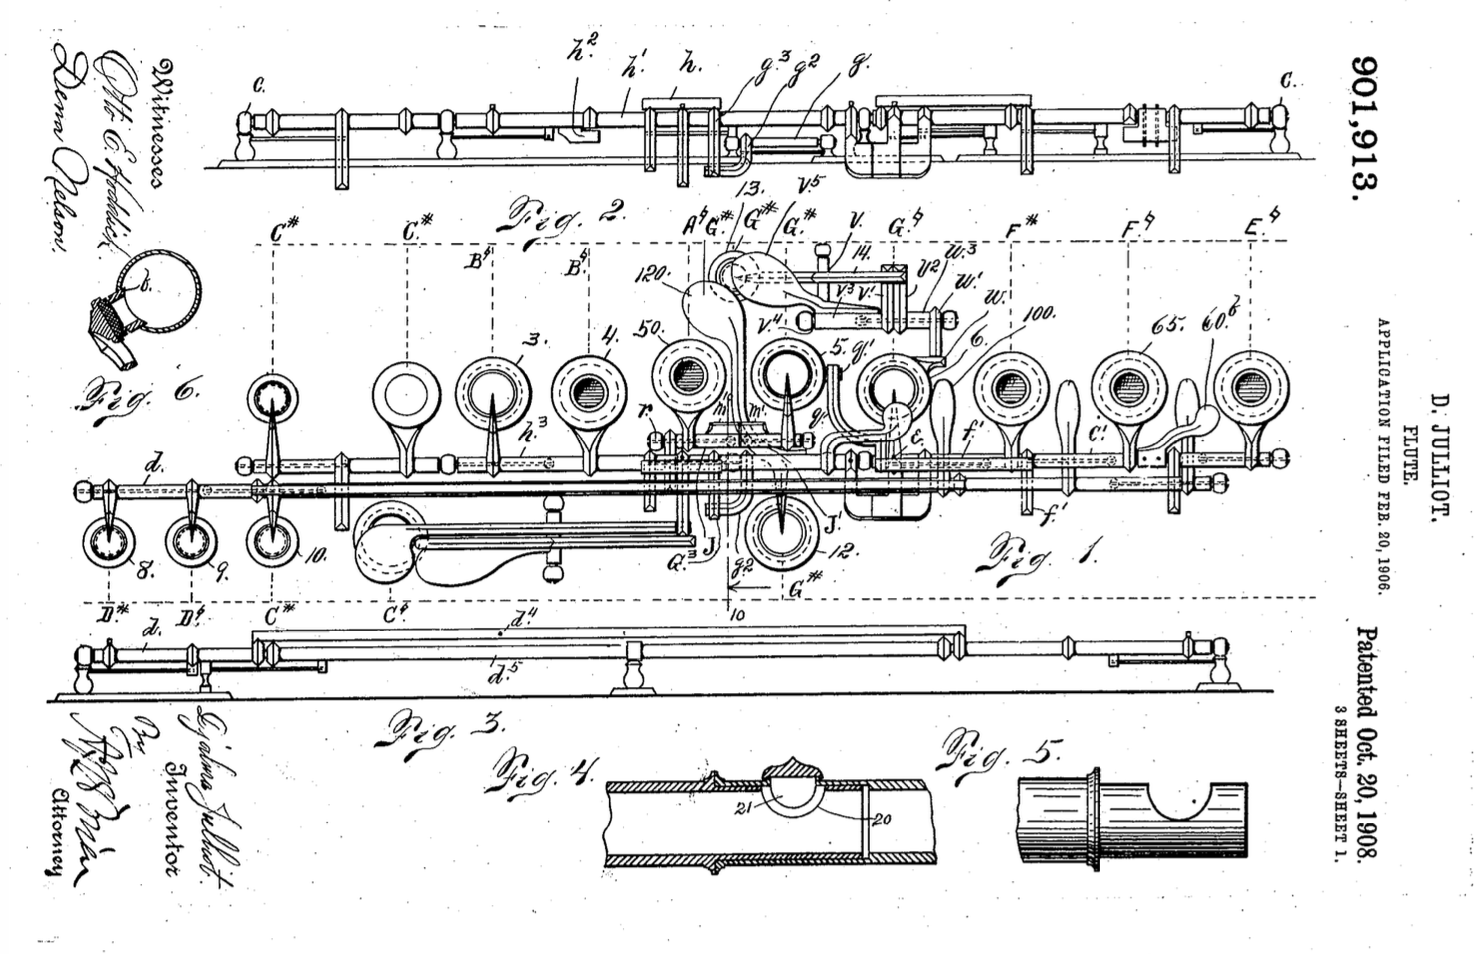
\includegraphics[width=\linewidth]{gfx/06_visual_representation/Julliot_patent.png}
	    \caption{Second caption}
	    \label{img2}
	\end{minipage}
\end{figure}


\begin{figure}
	\captionsetup{format =plain}%
	\centering
	\begin{minipage}[t]{0.48\textwidth}
		
\includegraphics[width=\linewidth]{gfx/06_visual_representation/f-hole.png}
		\caption{first figure but with more comments than the second picture to see what the different is.}
	\end{minipage}
	\hspace{.02\linewidth}
	\begin{minipage}[t]{0.48\textwidth}
	    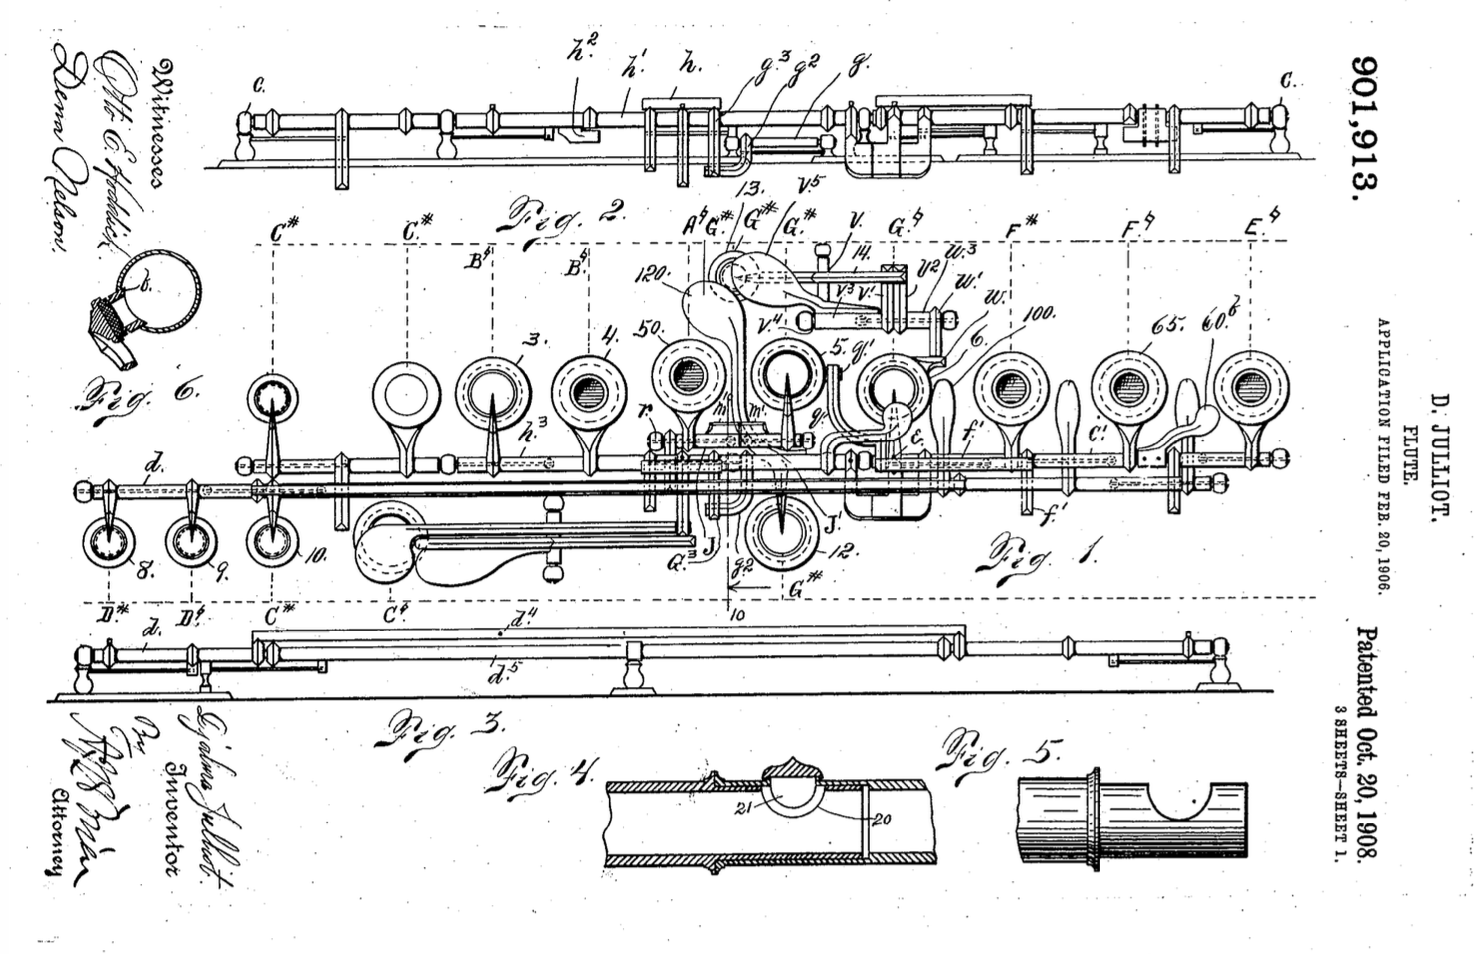
\includegraphics[width=\linewidth]{gfx/06_visual_representation/Julliot_patent.png}
		\caption{second figure}
	\end{minipage}
\end{figure}